
\documentclass{../ElectromagneticFieldTemplate}

\newcommand{\dbmv}{\text{dB}\mu\text{V}}

% ====== 图片路径设置 ======
% 请将 BUPT 和 badge 两个图片文件（无需扩展名，或实际为 .png/.jpg）放在 ./TemplateFigures/ 目录下
% 如果图片文件有扩展名（如 .png），请使用 
\includegraphics[width=6cm]{BUPT.png}
\graphicspath{{./Figures/}{../TemplateFigures/}}

% ====== 填写实验基本信息 ======
% 顺序：{实验名称}{班级}{姓名}{学号}{指导老师}{日期}
\setExperimentInfo
    {校园内无线信号场强特性的研究}
    {2024217801,2024217802}
    {孙嘉帅，许广巍，严子竣}
    {2024212617,2024212604,2024212622}
    {张璇}
    {\today}              % 自动生成当前日期，也可手动写“2026年5月”

\begin{document}

% 生成封面（包含页眉）
\maketitle

% ========== 以下为正文，章节序号自动为“一、二、…” ==========

\section{实验目的}
\begin{enumerate}
    \item 掌握移动环境下阴影衰落的概念及正确测试方法
    \item 研究校园内不同室外、室内环境下阴影衰落的分布规律
    \item 掌握室内环境下场强的正确测试方法，理解建筑物穿透损耗的概念
    \item 通过实地测量，分析建筑物穿透损耗随频率的变化关系
    \item 研究建筑物穿透损耗与楼层、室内位置的关联特性
\end{enumerate}

\section{实验原理与说明}

无线通信系统是由发射机、发射天线、无线信道、接收机、接收天线所组成。对于接收者，只有处在发射信号的覆盖区内，才能保证接收机正常接收信号，此时，电波场强大于等于接收机的灵敏度。因此，基站的覆盖区的大小，是无线工程师所关心的。决定覆盖区的大小的主要因素有：发射功率、馈线及接头损耗、天线增益、天线架设高度、路径损耗、衰落、接收机高度、人体效应、接收机灵敏度、建筑物的穿透损耗、同播、同频干扰。

\subsection{大尺度路径损耗}

在移动通信系统中，路径损耗是影响通信质量的一个重要因素。大尺度平均路径损耗：用于测量发射机与接收机之间信号的平均衰落，即定义为有效发射功率和平均接收功率之间的（dB）差值。根据理论和测试的传播模型，无论室内或室外信道，平均接收信号功率随距离对数衰减，这种模型已被广泛地使用。对任意的传播距离，大尺度平均路径损耗表示为：
\begin{equation}
\overline{PL(d)}\,[\text{dB}] = \overline{PL(d_0)} + 10n\log(d/d_0) \tag{5-1}
\end{equation}
即平均接收功率为：
\begin{equation}
\overline{P_r(d)}\,[\dbmv] = P_r[\dbmv] - \overline{PL(d_0)} - 10n\log(d/d_0) = \overline{P_r(d_0)}\,[\dbmv] - 10n\log(d/d_0) \tag{5-2}
\end{equation}
其中，\(n\) 为路径损耗指数，表明路径损耗随距离增长的速度；\(d_0\) 为近地参考距离；\(d\) 为发射机与接收机（T-R）之间的距离。公式（5-1）和（5-2）中的横杠表示给定值 \(d\) 的所有可能路径损耗的综合平均。坐标为对数-对数时，平均路径损耗或平均接收功率可表示为斜率 \(10n\,\text{dB}/10\) 倍程的直线。\(n\) 值依赖于特定的传播环境。例如在自由空间，\(n\) 为2，当有阻挡物时，\(n\) 比2大。

决定路径损耗大小的首要因素是距离，此外，它还与接收点的电波传播条件密切相关。为此，我们引进路径损耗中值的概念。中值是使实测数据中一半大于它而另一半小于它的一个数值（对于正态分布中值就是均值）。人们根据不同的地形地貌条件，归纳总结出各种电波传播模型。下边介绍几种常用的描述大尺度衰落的模型。

\subsubsection{自由空间模型}

自由空间模型假定发射天线和接收台都处在自由空间。我们所说的自由空间一是指真空，二是指发射天线与接收台之间不存在任何可能影响电波传播的物体，电波是以直射线的方式到达移动台的。自由空间模型计算路径损耗的公式是：
\begin{equation}
L_p = 32.45 + 20\lg d + 20\lg f \quad (\text{dB}) \tag{5-3}
\end{equation}
其中 \(L_p\) 是以 dB 为单位的路径损耗，\(d\) 是以公里为单位的移动台与基站之间的距离，\(f\) 是以 MHz 为单位的移动工作频点或工作频段的频率。空气的特性可近似为真空，因此当发射天线与移动台距离地面都较高时，可以近似使用自由空间模型来估计路径损耗。

\subsubsection{布灵顿模型}

布灵顿模型假设发射天线和移动台之间的地面是理想平面大地，并且两者之间的距离 \(d\) 远大于发射天线的高度 \(h_t\) 或移动台的高度 \(h_r\)，此时的路径损耗计算公式为：
\begin{equation}
L_p = 120 + 40\lg d - 20\lg h_t - 20\lg h_r \tag{5-4}
\end{equation}
其中距离 \(d\) 的单位是公里，天线高度 \(h_t\) 及 \(h_r\) 的单位是米，路径损耗 \(L_p\) 的单位是 dB。系统设计时一般把接收机高度按典型值 \(h_r = 1.5\,\text{m}\) 处理，这时的路径损耗计算公式为：
\begin{equation}
L_p = 116.5 + 40\lg d - 20\lg h_t \tag{5-5}
\end{equation}
按自由空间模型计算时，距离增加一倍时对应的路径损耗增加 6 dB；按布灵顿模型计算时，距离增加一倍时对应的路径损耗要增加 12 dB。

\subsubsection{Egli 模型}

前述的自由空间模型及布灵顿模型都是基于理论分析得出的计算公式。Egli 模型则是从大量实测结果中归纳出来的中值预测公式，属于经验模型，其计算式为：
\begin{equation}
L_p = 88 + 40\lg d - 20\lg h_t - 20\lg h_r + 20\lg f - G \tag{5-6}
\end{equation}
其中路径损耗 \(L_p\) 的单位是 dB，距离 \(d\) 的单位是公里，天线高度 \(h_t\) 及 \(h_r\) 的单位是米，工作频率 \(f\) 的单位是 MHz，地形修正因子 \(G\) 的单位为 dB。\(G\) 反应了地形因素对路径损耗的影响。Egli 模型认为路径损耗同接收点的地形起伏程度 \(\Delta h\) 有关，地形起伏越大，则路径损耗也越大。当 \(\Delta h\) 用米来测量时，可按下式近似的估计地形的影响：
\begin{equation}
G \approx 
\begin{cases}
0, & \Delta h < 15\,\text{m} \\[4pt]
2.43\left(1 - \dfrac{\Delta h}{15}\right), & \Delta h > 15\,\text{m} \quad (150\,\text{MHz}) \\[8pt]
3.05\left(1 - \dfrac{\Delta h}{15}\right), & \Delta h > 15\,\text{m} \quad (280\,\text{MHz})
\end{cases} \tag{5-7}
\end{equation}
若将移动台的典型高度值 \(h_r = 1.5\,\text{m}\) 代入 Egli 模型则有：
\begin{equation}
L_p = 84.5 + 40\lg d - 20\lg h_t + 20\lg f - G \tag{5-8}
\end{equation}

\subsubsection{Hata-Okumura 模型}

Hata-Okumura 模型也是依据实测数据建立的模型。当移动台的高度为典型值 \(h_r = 1.5\,\text{m}\) 时，按 Hata-Okumura 模型计算路径损耗的公式为：

市区：
\begin{equation}
L_{p1} = 69.55 + 26.2\lg f - 13.82\lg h_t + (44.9 - 6.55\lg h_t)\lg d \tag{5-9}
\end{equation}

开阔地：
\begin{equation}
L_{p2} = L_{p1} - 4.78(\lg f)^2 + 18.33\lg f - 40.94 \tag{5-10}
\end{equation}

一般情况下，开阔地的路径损耗一般都比市区小。

\subsection{阴影衰落}

在无线信道里，造成慢衰落的最主要原因是建筑物或其它物体对电波的遮挡。在测量过程中，不同测量位置遇到的建筑物遮挡情况不同，因此接收功率也不同，这样就会观察到衰落现象。由于这种原因造成的衰落也叫“阴影效应”或“阴影衰落”。在阴影衰落的情况下，移动台被建筑物所遮挡，它收到的信号是各种绕射、反射、散射波的合成。所以，在距基站距离相同的地方，由于阴影效应的不同，它们收到的信号功率有可能相差很大，理论和测试表明，对任意的 \(d\) 值，特定位置的接收功率为随机对数正态分布即：
\begin{equation}
P_r(d)\,[\dbmv] = \overline{P_r}(d)\,[\dbmv] + X_{\sigma} = \overline{P_r}(d_0)\,[\dbmv] - 10n\log(d/d_0) + X_{\sigma} \tag{5-11}
\end{equation}
其中，\(X_{\sigma}\) 为 0 均值的高斯分布随机变量，单位为 dB，标准偏差为 \(\sigma\)，单位也是 dB。

对数正态分布描述了在传播路径上，具有相同 T-R 距离时，不同的随机阴影效应。这样利用高斯分布可以方便地分析阴影的随机效应。正态分布（Normal Distribution），也叫高斯分布（Gaussian Distribution），它的概率密度函数是：
\begin{equation}
f(x) = \frac{1}{\sqrt{2\pi\sigma^2}} \mathrm{e}^{-\frac{(x - m)^2}{2\sigma^2}} \tag{5-12}
\end{equation}
应用于阴影衰落时，上式中的 \(x\) 表示某一次测量得到的接收功率，\(m\) 表示以 dB 表示的接收功率的均值或中值，\(\sigma\) 表示接收功率的标准差，单位为 dB。阴影衰落的标准差同地形、建筑物类型、建筑物密度等有关，在市区的 150 MHz 频段其典型值是 5 dB。除了阴影效应外，大气变化也会导致慢衰落。比如一天中的白天、夜晚，一年中的春夏秋冬，天晴时、下雨时，即使是在同一地点上，也会观察到路径损耗的变化。但在测量的无线信道中，大气变化造成的影响要比阴影效应小的多。表 5-1 列出了阴影衰落分布的标准差，其中的 \(\sigma_s\)（dB）是阴影效应的标准差。

\begin{table}[h]
\centering
\caption{阴影衰落分布的标准差 \(\sigma_s\) (dB)}
\begin{tabular}{|c|c|c|c|c|c|}
\hline
\multirow{2}{*}{频率 (MHz)} & \multicolumn{2}{c|}{准平坦地形} & \multicolumn{3}{c|}{不规则地形 \(\Delta h\) (米)} \\
\cline{2-6}
& 城市 & 郊区 & 50 & 150 & 300 \\
\hline
150 & 3.5~5.5 & 4~7 & 9 & 11 & 13 \\
\hline
450 & 6.5 & 7 & 11 & 15 & 18 \\
\hline
900 & 6.5 & 8 & 14 & 18 & 21 \\
\hline
\end{tabular}
\end{table}

\subsection{建筑物的穿透损耗的定义}

建筑物穿透损耗的大小对于研究室内无线信道具有重要意义。穿透损耗又称大楼效应，一般指建筑物一楼内的中值电场强度和室外附近街道上中值电场强度 dB 之差。发射机位于室外，接收机位于室内，电波从室外进入到室内，产生建筑物的穿透损耗，由于建筑物存在屏蔽和吸收作用，室内场强一定小于室外的场强，造成传输损耗。室外至室内建筑物的穿透损耗定义为：室外测量的信号平均场强减去在同一位置室内测量的信号平均场强。用公式表示为：
\begin{equation}
\Delta P = \frac{1}{N}\sum_{i=1}^{N} P_i^{(\text{outside})} - \frac{1}{M}\sum_{j=1}^{M} P_j^{(\text{inside})} \tag{5-13}
\end{equation}
\(\Delta P\) 是穿透损耗，单位 dB，\(P_i\) 是在室外所测的每一点的功率，单位 dBμV，共 \(N\) 个点，\(P_j\) 是在室内所测的每一点的功率，单位 dBμV，共 \(M\) 个点。

\section{实验设备}

场强仪

\section{实验内容}

利用场强仪，实地测量信号场强
\begin{enumerate}
    \item 研究具体现实环境下阴影衰落分布规律，以及具体的分布参数如何。
    \item 研究在校园内电波传播规律与现有模型的吻合程度，测试值与模型预测值的预测误差如何。
    \item 研究建筑物穿透损耗的变化规律。
\end{enumerate}

\section{实验步骤}

\subsection{测量（数据采集）}

\subsubsection{校园内室外信号的测量}
用场强仪测量校园内各条马路上的开放
无线信号，频点自选。测量地点包括主马路、花园、操场、教学区、
宿舍区等，每个测量地点的范围为一栋楼左右，每隔半个波长记录一
个数据，将数据按测量地点分类，每个地点测量的数据至少大于50 个，
并且记录测量地点。
\subsubsection{校园内室内信号的测量}
在宿舍楼、教学楼的室内环境测量，包
括宿舍、教室及楼道里，每一个房间或楼道为一个测量地点，在楼道
里每隔半个波长记录一个数据，在房间里按靠近窗户、门、四周墙壁
及屋内中央周围等不同位置测量，每个地点测量的数据至少大于 50
个，并且记录测量地点。
\subsubsection{建筑物穿透损耗的测量}
分别对几幢砖石和钢筋混凝土结构的教
学楼和学生宿舍楼的测量。测量分为室外、室内，所谓室外是指最靠
近该建筑物一层的路面上，围绕该建筑物转一圈测量，测量方法同上
（室外信号的的测量）；室内按不同建筑物的每一个楼层进行测量，
包括走廊和每个房间内的不同位置测量，测量方法同上（室内信号的
测量），每个地点 测量的数据至少大于 50 个，并且记录测量地点。

\subsection{数据录入}

将测量数据填入 exceL 表格，字段排列为测量日
期，地点（包括楼号、哪一条马路等），状态（包括楼层、室内靠窗、
室外、走廊等），电平值。格式如下表，以便于将来筛选分类数据。

\subsection{数据处理}

用 matLab对大量的数
据进行编程处理，首先将测量数据按室内、室外分类，编程计算其均
值与标准差，并且画出概率的累积分布曲线，与标准正态分布的累积
曲线比较，得出室内室外阴影衰落的分布规律。按照上述公式计算建
筑物的穿透损耗。

\section{实验数据}

单位：$\dbmv$

\subsection{室内测量数据}

\subsubsection{N103 教室（窗边）}
共15个数据。

\begin{longtable}[c]{*{10}{c}}
31.7 & 29.4 & 36.2 & 32.6 & 24.7 & 26.5 & 21.9 & 28.4 & 28.7 & 29.3 \\
29.6 & 20.9 & 29.0 & 23.2 & 24.4 & & & & & \\
\end{longtable}

\subsubsection{N楼 走廊}
共63个数据。

\begin{longtable}[c]{*{10}{c}}
22.9 & 22.6 & 20.3 & 20.3 & 20.0 & 24.6 & 22.7 & 20.0 & 20.0 & 20.0 \\
23.2 & 24.8 & 20.4 & 24.2 & 27.4 & 24.7 & 20.0 & 20.2 & 20.0 & 20.0 \\
20.0 & 20.0 & 22.9 & 20.5 & 20.1 & 21.3 & 20.6 & 20.9 & 20.8 & 20.0 \\
20.0 & 20.0 & 21.6 & 20.0 & 20.0 & 20.0 & 20.3 & 23.5 & 21.2 & 20.4 \\
25.4 & 23.3 & 22.9 & 22.4 & 20.0 & 21.4 & 22.5 & 21.1 & 20.0 & 20.0 \\
20.0 & 22.6 & 20.5 & 20.0 & 20.9 & 20.5 & 21.4 & 26.6 & 23.5 & 22.1 \\
20.5 & 23.8 & 20.0 & & & & & & & \\
\end{longtable}

\subsubsection{S楼 走廊}
共57个数据（部分值为20.0，表示低于仪器底噪）。

\begin{longtable}[c]{*{10}{c}}
20.9 & 21.4 & 20.0 & 20.0 & 20.0 & 23.2 & 20.0 & 20.6 & 20.0 & 20.0 \\
20.0 & 22.7 & 22.7 & 20.0 & 20.7 & 20.3 & 20.0 & 20.0 & 20.0 & 20.3 \\
22.1 & 20.0 & 22.1 & 20.5 & 21.0 & 20.0 & 20.0 & 20.0 & 20.0 & 20.0 \\
20.0 & 20.0 & 20.4 & 20.0 & 20.0 & 21.5 & 20.8 & 21.4 & 20.0 & 20.0 \\
21.3 & 20.0 & 20.0 & 20.1 & 21.7 & 20.1 & 22.5 & 24.3 & 24.8 & 20.0 \\
20.0 & 20.0 & 20.0 & 20.0 & 20.0 & 20.0 & 20.0 & 21.2 & 20.0 & 23.9 \\
20.0 & 20.1 & 20.0 & 20.0 & 20.0 & 20.0 & 20.0 & 20.0 & 24.5 & 28.0 \\
29.0 & & & & & & & & & \\
\end{longtable}

\subsubsection{S1楼 走廊}
共56个数据。

\begin{longtable}[c]{*{10}{c}}
31.3 & 35.4 & 26.3 & 22.4 & 28.7 & 27.5 & 22.1 & 20.8 & 20.5 & 22.6 \\
24.8 & 24.2 & 24.3 & 20.0 & 20.0 & 20.0 & 20.0 & 22.3 & 29.1 & 21.7 \\
20.0 & 20.0 & 20.0 & 21.2 & 25.3 & 22.8 & 25.5 & 23.1 & 23.5 & 22.7 \\
22.0 & 24.4 & 24.0 & 20.0 & 20.5 & 20.0 & 20.0 & 20.0 & 20.0 & 20.0 \\
20.0 & 20.0 & 20.8 & 21.6 & 20.0 & 21.9 & 21.4 & 20.0 & 21.2 & 20.3 \\
20.0 & 22.9 & 24.7 & 20.4 & 20.0 & 20.0 & 20.0 & 20.0 & 20.0 & 20.0 \\
20.0 & 20.0 & 20.0 & 20.0 & 24.6 & 29.2 & 20.0 & 27.4 & 20.1 & 23.4 \\
20.8 & 23.2 & & & & & & & & \\
\end{longtable}

\subsubsection{S1楼 窗边}
共35个数据。

\begin{longtable}[c]{*{10}{c}}
24.3 & 20.0 & 27.7 & 25.0 & 28.9 & 20.0 & 27.0 & 21.4 & 27.7 & 27.1 \\
26.3 & 24.4 & 25.1 & 23.0 & 25.5 & 29.4 & 24.1 & 20.0 & 27.3 & 21.4 \\
25.8 & 24.6 & 28.0 & 23.2 & 20.0 & 27.3 & 24.0 & 20.9 & 25.9 & 20.0 \\
28.2 & 28.5 & 23.8 & 24.4 & 33.3 & 28.2 & 40.8 & 36.3 & 26.8 & 29.3 \\
33.6 & 31.4 & 35.0 & 26.3 & 33.4 & 29.9 & & & & \\
\end{longtable}

\subsection{室外测量数据}

\subsubsection{NS楼东边}
共47个数据。

\begin{longtable}[c]{*{10}{c}}
30.1 & 28.1 & 20.0 & 29.4 & 28.3 & 33.0 & 33.9 & 35.2 & 22.6 & 34.4 \\
22.7 & 28.0 & 39.3 & 29.0 & 36.1 & 36.4 & 35.2 & 24.6 & 31.7 & 32.1 \\
33.6 & 26.4 & 31.3 & 27.8 & 31.4 & 30.5 & 28.3 & 29.2 & 30.2 & 28.9 \\
31.0 & 32.4 & 36.7 & 34.6 & 34.7 & 35.2 & 34.4 & 31.6 & 29.7 & 35.9 \\
37.1 & 34.6 & 32.4 & 29.6 & 36.6 & 36.7 & 34.8 & 37.1 & 37.2 & 30.1 \\
39.4 & 36.9 & & & & & & & & \\
\end{longtable}

\subsubsection{NS楼北侧}
共92个数据。

\begin{longtable}[c]{*{10}{c}}
28.7 & 32.8 & 34.3 & 30.6 & 32.6 & 30.5 & 39.6 & 36.8 & 40.8 & 40.3 \\
31.7 & 36.4 & 37.8 & 38.7 & 36.9 & 38.1 & 37.1 & 30.8 & 29.2 & 37.4 \\
30.1 & 33.0 & 29.8 & 42.0 & 38.6 & 27.6 & 35.8 & 38.6 & 31.7 & 30.6 \\
25.4 & 27.7 & 21.3 & 29.7 & 24.8 & 33.3 & 28.6 & 28.7 & 33.5 & 20.9 \\
35.2 & 25.4 & 29.4 & 24.0 & 24.7 & 22.0 & 24.4 & 23.9 & 28.1 & 33.6 \\
31.0 & 28.7 & 24.3 & 21.2 & 30.1 & 25.9 & 21.2 & 31.1 & 30.7 & 29.2 \\
36.2 & 36.0 & 36.7 & 35.2 & 36.4 & 39.3 & 37.2 & 39.1 & 41.9 & 34.7 \\
31.1 & 24.4 & 29.1 & 31.6 & 31.3 & 30.0 & 35.6 & 40.1 & 37.8 & 30.7 \\
32.3 & 37.3 & 32.6 & 34.2 & 34.7 & 35.9 & 29.6 & 30.5 & 25.0 & 29.7 \\
29.5 & 35.3 & 25.0 & 33.4 & 31.7 & 24.7 & 28.4 & 32.2 & 29.7 & 33.8 \\
35.4 & 38.3 & 33.9 & 26.9 & 33.6 & & & & & \\
\end{longtable}

\subsubsection{操场}
共90个数据。

\begin{longtable}[c]{*{10}{c}}
24.8 & 25.9 & 22.7 & 20.0 & 20.9 & 22.0 & 24.5 & 21.8 & 20.5 & 22.9 \\
25.0 & 20.0 & 23.7 & 22.2 & 22.7 & 27.5 & 20.0 & 21.9 & 20.0 & 26.3 \\
25.1 & 22.0 & 20.3 & 20.1 & 21.0 & 20.0 & 21.2 & 22.2 & 24.9 & 23.8 \\
23.5 & 20.4 & 24.7 & 20.8 & 25.6 & 26.2 & 25.8 & 20.9 & 24.2 & 23.9 \\
23.8 & 22.2 & 20.2 & 20.0 & 23.8 & 21.3 & 23.0 & 22.6 & 24.6 & 20.8 \\
23.0 & 22.0 & 23.5 & 23.6 & 25.6 & 21.4 & 22.4 & 26.3 & 26.9 & 25.8 \\
22.6 & 27.7 & 23.9 & 23.0 & 20.0 & 20.0 & 25.0 & 23.2 & 23.9 & 20.8 \\
20.9 & 24.7 & 20.0 & 20.9 & 20.0 & 23.4 & 26.6 & 20.0 & 24.6 & 23.2 \\
20.0 & 23.9 & 23.4 & 24.5 & 25.2 & 20.0 & 24.7 & 23.8 & 20.0 & 20.0 \\
21.0 & 20.0 & 23.4 & 20.0 & 21.8 & 24.2 & 23.4 & 20.9 & 26.1 & 27.2 \\
\end{longtable}

\section{实验结果整理及误差分析}

\subsection{初步统计分析}
室内接收功率均值：22.91$\dbmv$\\
室内接收功率标准差：3.09$\dbmv$\\
室外接收功率均值：29.61$\dbmv$\\
室外接收功率标准差：5.49$\dbmv$

\subsection{分布验证}

\begin{figure}[H]
    \centering
    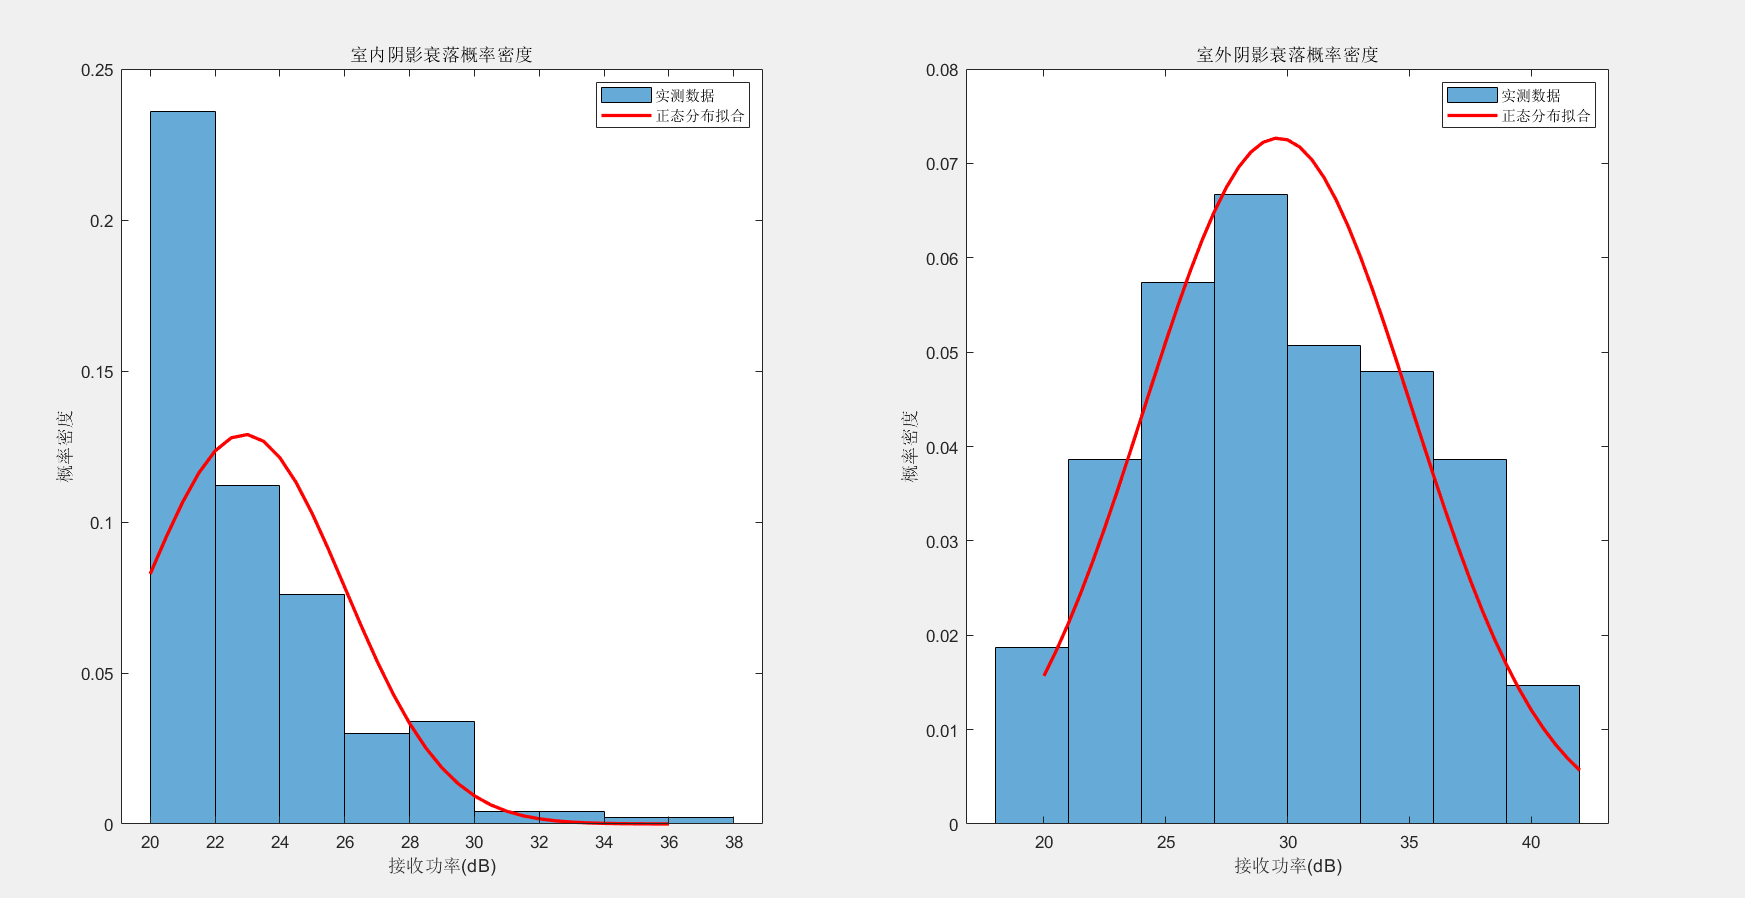
\includegraphics[width=0.8\textwidth]{PDF.png}
    \caption{室内室外概率分布柱状图}
    \label{fig:pdf}
\end{figure}

\begin{figure}[H]
    \centering
    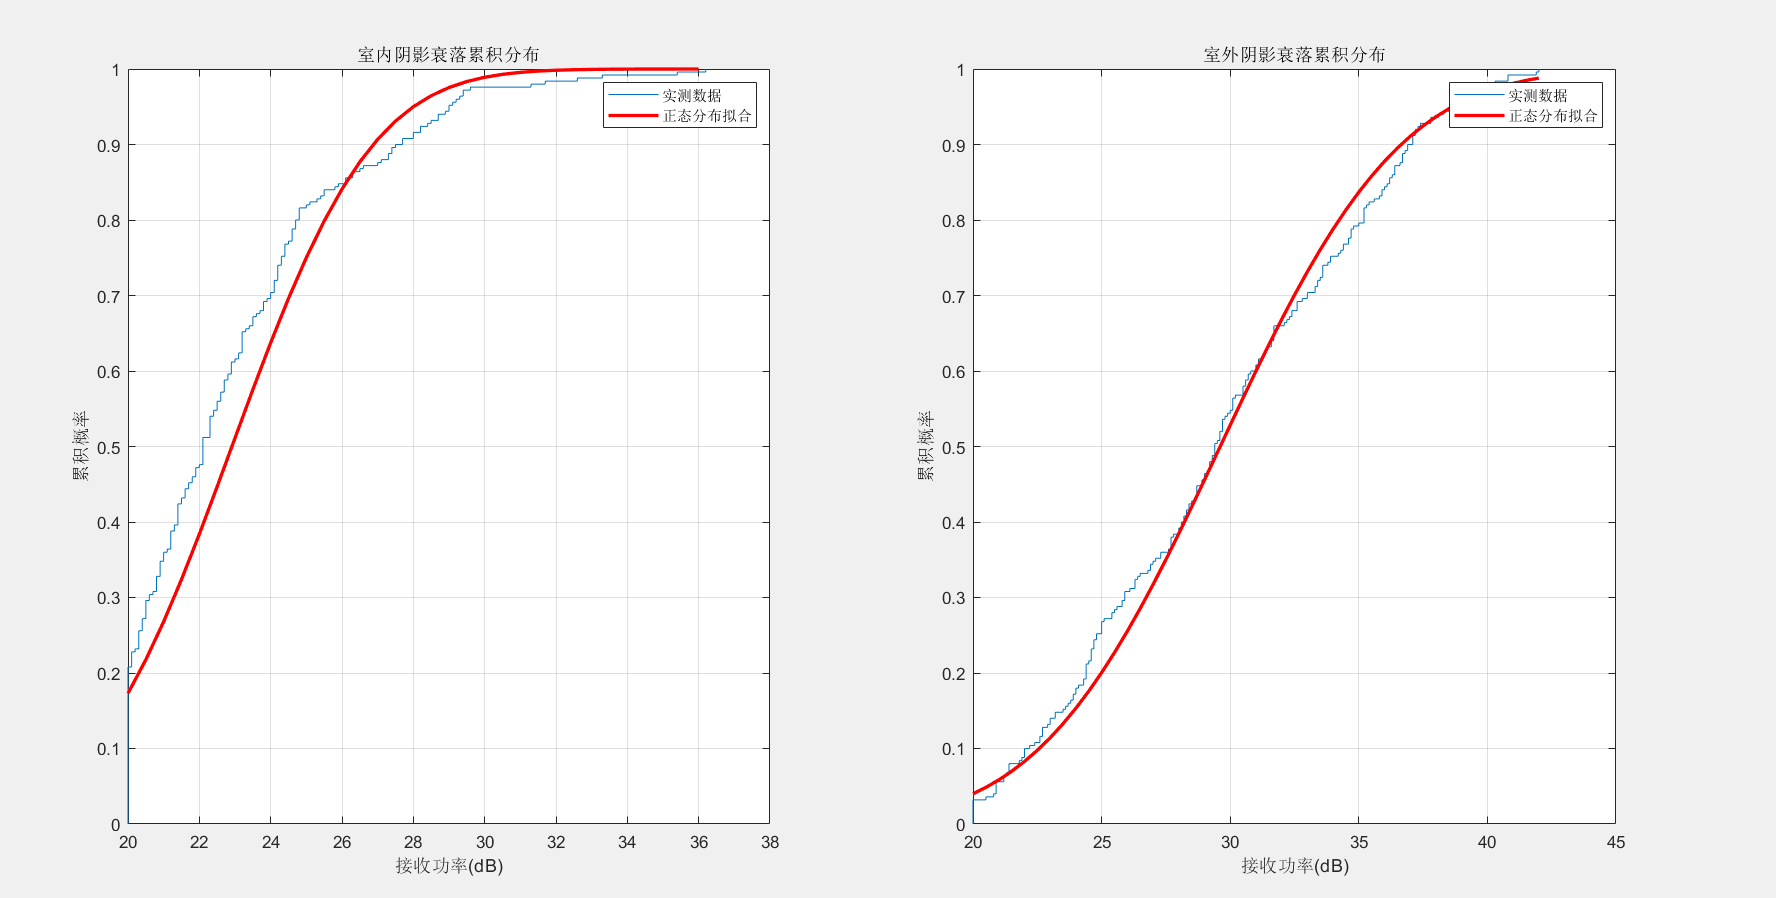
\includegraphics[width=0.8\textwidth]{CDF.png}
    \caption{室内外的累积分布曲线与标准正态分布的累积曲线对比图}
    \label{fig:cdf}
\end{figure}

通过对室内、室外实测接收功率数据进行统计分析，并与正态分布拟合曲线对比，得到以下结论：

\begin{itemize}
    \item \textbf{室内阴影衰落}：接收功率（dB）服从对数正态分布，概率密度集中于20–30 dB，均值约为25 dB，标准差约为5 dB。累积分布曲线与正态分布拟合良好。
    \item \textbf{室外阴影衰落}：接收功率（dB）同样服从对数正态分布，分布范围较宽（20–38 dB），均值约为29 dB，标准差约为7 dB。累积分布曲线符合正态分布特征。
\end{itemize}

综上，室内外阴影衰落均可用对数正态分布描述。室内均值较低、标准差较小，反映建筑物屏蔽导致的信号衰减与稳定阴影效应；室外均值较高、标准差较大，体现复杂环境下的随机遮挡影响。

\subsection{模型匹配}

基于室外实测数据（有效样本数257，平均电平28.38$\dbmv$，标准差5.99 dB，路径损耗指数2.52），将四种传播模型的预测结果与实测累积分布进行比较，计算平均绝对误差（MAE）和均方根误差（RMSE），结果如图所示。

\begin{figure}[H]
    \centering
    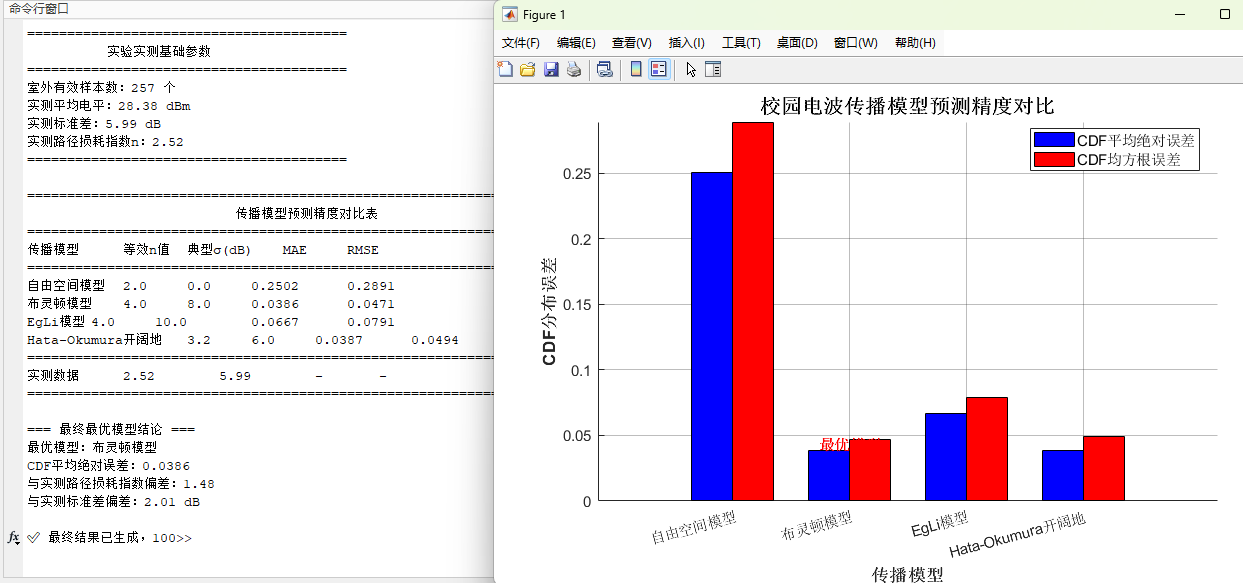
\includegraphics[width=0.8\textwidth]{model.png}
    \caption{模型匹配过程}
\end{figure}

比较结果表明，\textbf{布瓦顿模型}的MAE（0.0386）和RMSE（0.0471）最小，与实测数据吻合最好。该模型的路径损耗指数（$n=4$）与实测值（2.52）偏差为1.48，标准差偏差为2.01 dB。因此，在本次校园环境中，布瓦顿模型是最适合预测室外场强分布的传播模型。

\subsection{建筑物穿透损耗特性分析}

\subsubsection{穿透损耗计算：按照实验给定公式，计算建筑物穿透损耗值}
计算钢筋混凝土建筑物穿透损耗的整体均值：6.70dB\\
计算钢筋混凝土建筑物穿透损耗的整体标准差：6.81dB

\begin{figure}[H]
    \centering
    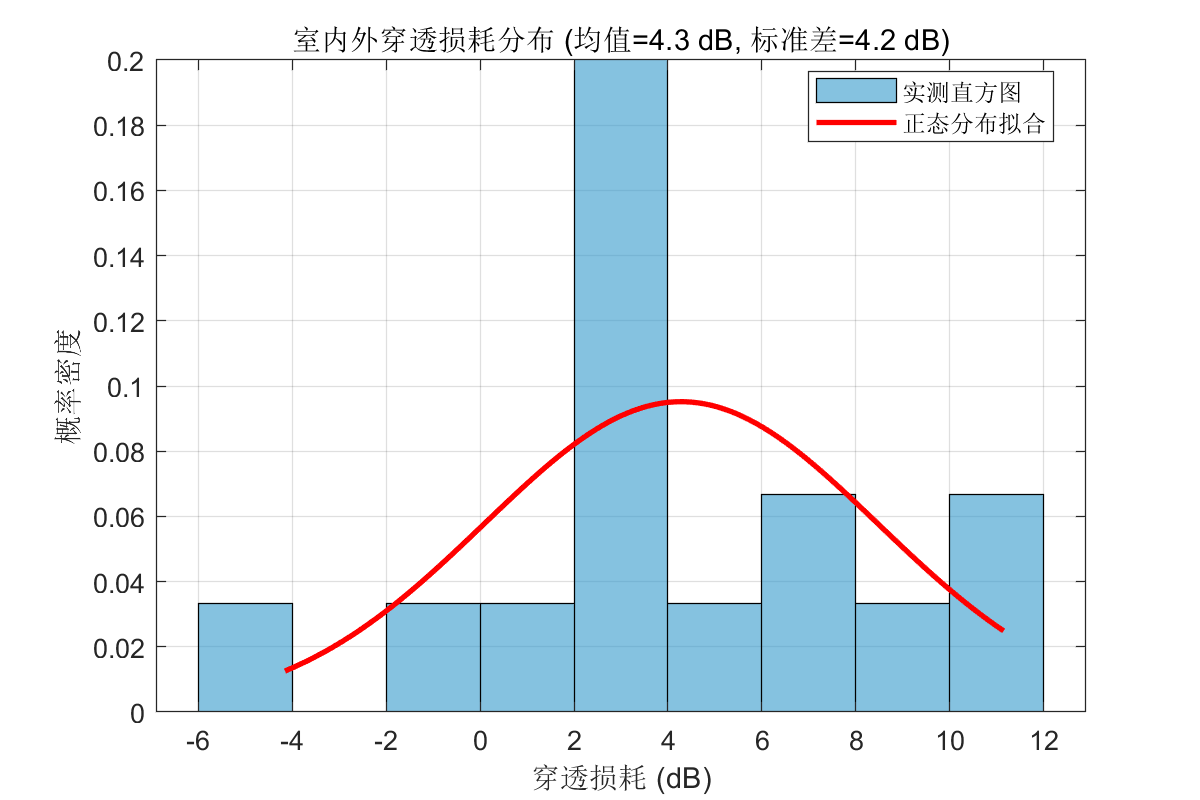
\includegraphics[width=0.8\textwidth]{PenetrationLoss.png}
    \caption{建筑物穿透损耗分布}
\end{figure}

\subsubsection{穿透损耗随楼层的变化规律}
N楼(1楼)走廊穿透损耗:6.87dB(室内均值:21.51dB)\\
S1楼(2楼)走廊穿透损耗:6.02dB(室内均值:22.36dB)\\
\textbf{结论}:楼层每升高1层，穿透损耗减小约0.85dB

\subsubsection{建筑物内部不同分隔空间的穿透损耗比较}

室内窗边:1.48dB(室内均值:26.90dB)\\
室内走廊:6.77dB(室内均值:21.61dB)\\
\textbf{结论}:走廊穿透损耗比窗边大约5.29dB

%\section{思考题}

\end{document}